\usetikzlibrary{arrows.meta,positioning,fit,shapes.geometric}
\begin{figure}[htbp]
\centering
\begin{adjustbox}{max width=\linewidth,max totalheight=0.64\textheight,keepaspectratio}
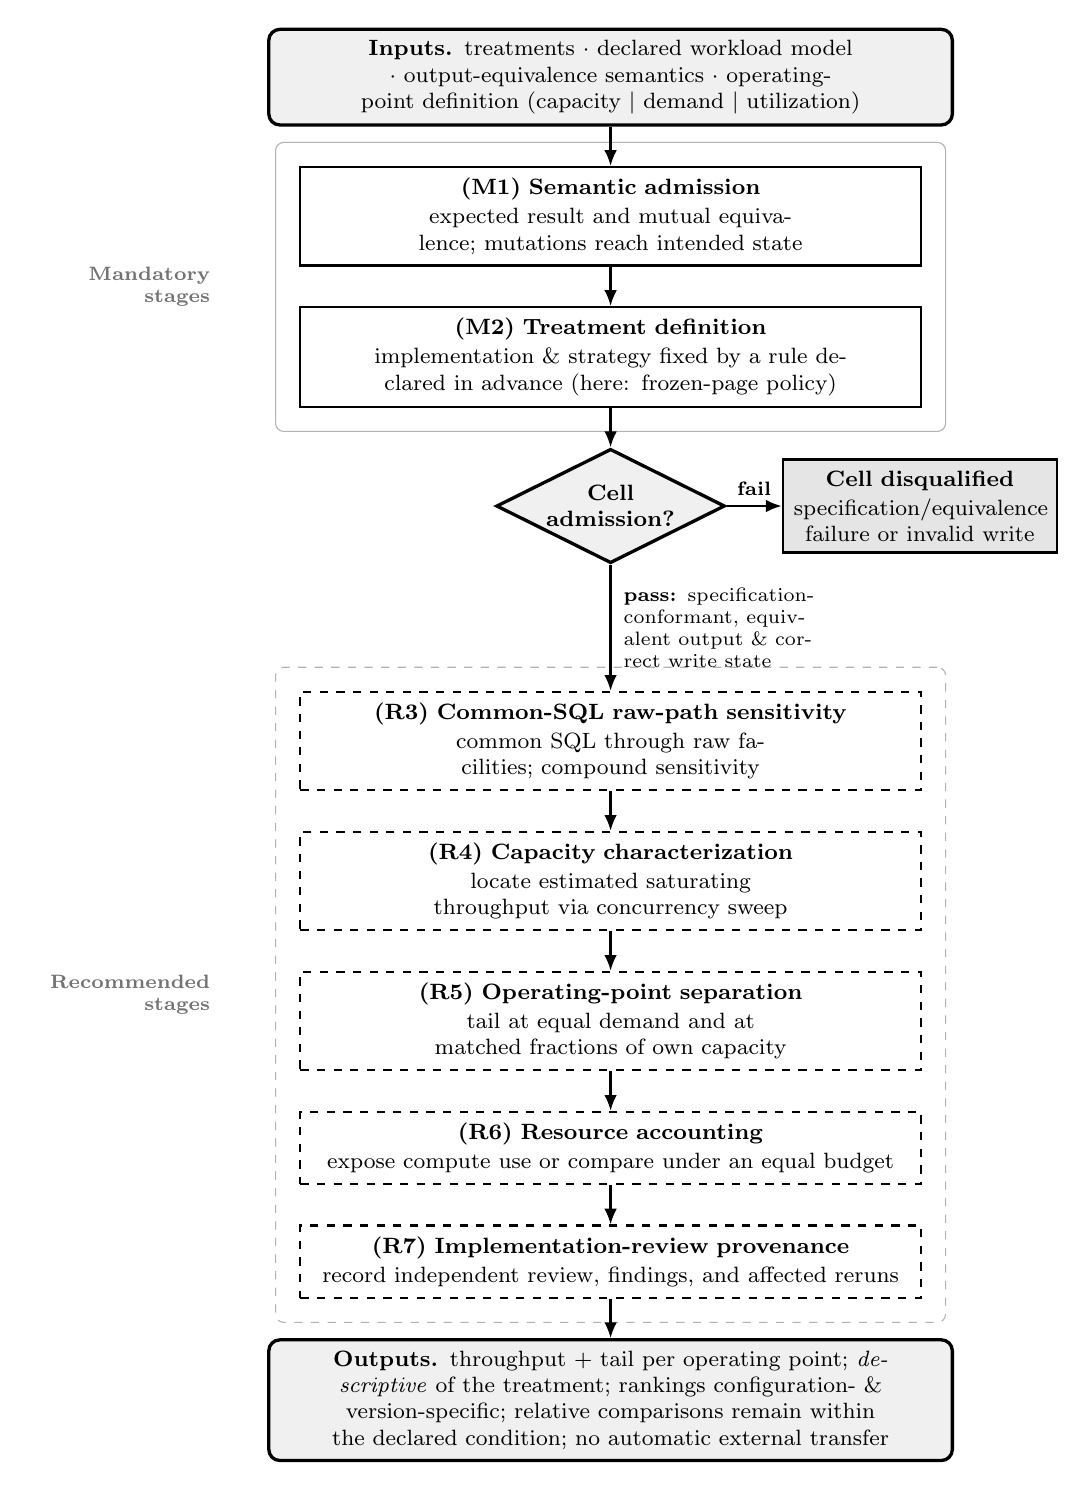
\begin{tikzpicture}[
  font=\footnotesize,
  node distance=5mm and 7mm,
  io/.style={rectangle, rounded corners=4pt, draw=black, very thick, fill=black!6,
             align=center, inner sep=4pt, text width=8.4cm},
  mand/.style={rectangle, draw=black, thick, fill=white,
               align=center, inner sep=4pt, text width=7.6cm},
  rec/.style={rectangle, draw=black, thick, dashed, fill=white,
              align=center, inner sep=4pt, text width=7.6cm},
  gate/.style={diamond, aspect=2, draw=black, very thick, fill=black!6,
               align=center, inner sep=1pt},
  reject/.style={rectangle, draw=black, thick, fill=black!10,
                 align=center, inner sep=4pt, text width=3.2cm},
  grp/.style={rounded corners=3pt, draw=black!30, inner sep=3mm},
  glab/.style={font=\scriptsize\bfseries, text width=2.2cm, align=right, black!55},
  arr/.style={-{Latex[length=2mm,width=1.6mm]}, thick},
]
% --- INPUTS ---
\node[io] (in) {\textbf{Inputs.} treatments $\cdot$ declared workload model $\cdot$
  output-equivalence semantics $\cdot$ operating-point definition
  (capacity $\mid$ demand $\mid$ utilization)};
% --- MANDATORY stages (solid) ---
\node[mand, below=of in] (m1) {\textbf{(M1)~Semantic admission}\\[1pt]
  expected result and mutual equivalence; mutations reach intended state};
\node[mand, below=of m1] (m2) {\textbf{(M2)~Treatment definition}\\[1pt]
  implementation \& strategy fixed by a rule declared in advance
  (here: frozen-page policy)};
% --- CELL-ADMISSION gate (decision) ---
\node[gate, below=of m2] (g) {\textbf{Cell}\\\textbf{admission?}};
% --- RECOMMENDED stages (dashed) ---
\node[rec, below=16mm of g] (r3) {\textbf{(R3)~Common-SQL raw-path sensitivity}\\[1pt]
  common SQL through raw facilities; compound sensitivity};
\node[rec, below=of r3] (r4) {\textbf{(R4)~Capacity characterization}\\[1pt]
  locate estimated saturating throughput via concurrency sweep};
\node[rec, below=of r4] (r5) {\textbf{(R5)~Operating-point separation}\\[1pt]
  tail at equal demand and at matched fractions of own capacity};
\node[rec, below=of r5] (r6) {\textbf{(R6)~Resource accounting}\\[1pt]
  expose compute use or compare under an equal budget};
\node[rec, below=of r6] (r7) {\textbf{(R7)~Implementation-review provenance}\\[1pt]
  record independent review, findings, and affected reruns};
% --- OUTPUTS ---
\node[io, below=of r7] (out) {\textbf{Outputs.} throughput $+$ tail per operating point;
  \emph{descriptive} of the treatment; rankings configuration- \& version-specific;
  relative comparisons remain within the declared condition; no automatic external transfer};
% --- disqualification branch ---
\node[reject, right=of g] (rej)
  {\textbf{Cell disqualified}\\[1pt] specification/equivalence failure
   or invalid write};
% --- group brackets + side labels ---
\node[grp, fit=(m1)(m2)] (mg) {};
\node[grp, dashed, fit=(r3)(r4)(r5)(r6)(r7)] (rg) {};
\node[glab, left=of mg] {Mandatory stages};
\node[glab, left=of rg] {Recommended stages};
% --- flow ---
\draw[arr] (in) -- (m1);
\draw[arr] (m1) -- (m2);
\draw[arr] (m2) -- (g);
\draw[arr] (g) -- node[right=1pt, text width=2.5cm, font=\scriptsize, align=left]
  {\textbf{pass:} specification-conformant, equivalent output \& correct write state} (r3);
\draw[arr] (r3) -- (r4);
\draw[arr] (r4) -- (r5);
\draw[arr] (r5) -- (r6);
\draw[arr] (r6) -- (r7);
\draw[arr] (r7) -- (out);
\draw[arr] (g) -- node[above, font=\scriptsize\bfseries]{fail} (rej);
\end{tikzpicture}
\end{adjustbox}
\caption{The comparability protocol. Semantic admission (M1) and treatment definition (M2) form the
  mandatory core. The recommended stages R3--R7 license common-SQL, capacity, utilization, resource,
  and implementation-provenance interpretations, and may be scoped to a representative workload point
  rather than the full matrix. A finite gate supplies task-conformance evidence; it does not prove
  arbitrary-input correctness. For reporting compliance, M1 and M2 together form one mandatory
  validity-core level and R3--R7 define five claim-specific extensions, giving the six-level scheme of
  Supplement Table~S40.}
\label{fig:protocol}
\end{figure}
